%----------------------------------------------------------------------------------------
%	PACKAGES AND OTHER DOCUMENT CONFIGURATIONS
%----------------------------------------------------------------------------------------

\documentclass[12pt]{article}

\usepackage{polski}
\usepackage[polish]{babel} 
\usepackage[utf8]{inputenc}
\usepackage{graphicx}
\usepackage{color}
\usepackage{listings}
\usepackage{geometry} 
\geometry{
 	a4paper, 
 	left	=20mm,
 	right	=20mm,
 	top		=20mm,
 	bottom	=20mm,
}
 
\definecolor{codegreen}{rgb}{0,0.6,0}
\definecolor{codegray}{rgb}{0.5,0.5,0.5}
\definecolor{codepurple}{rgb}{0.58,0,0.82}
\definecolor{backcolour}{rgb}{0.95,0.95,0.92}
 
\lstdefinestyle{mystyle}{
    backgroundcolor=\color{backcolour},   
    commentstyle=\color{codegreen},
    keywordstyle=\color{magenta},
    numberstyle=\tiny\color{codegray},
    stringstyle=\color{codepurple},
    basicstyle=\tiny,
    breakatwhitespace=false,         
    breaklines=true,                 
    captionpos=b,                    
    keepspaces=true,                 
    numbers=left,                    
    numbersep=5pt,                  
    showspaces=false,                
    showstringspaces=false,
    showtabs=false,                  
    tabsize=2  
}
 
%----------------------------------------------------------------------------------------

\begin{document}

\begin{center}
	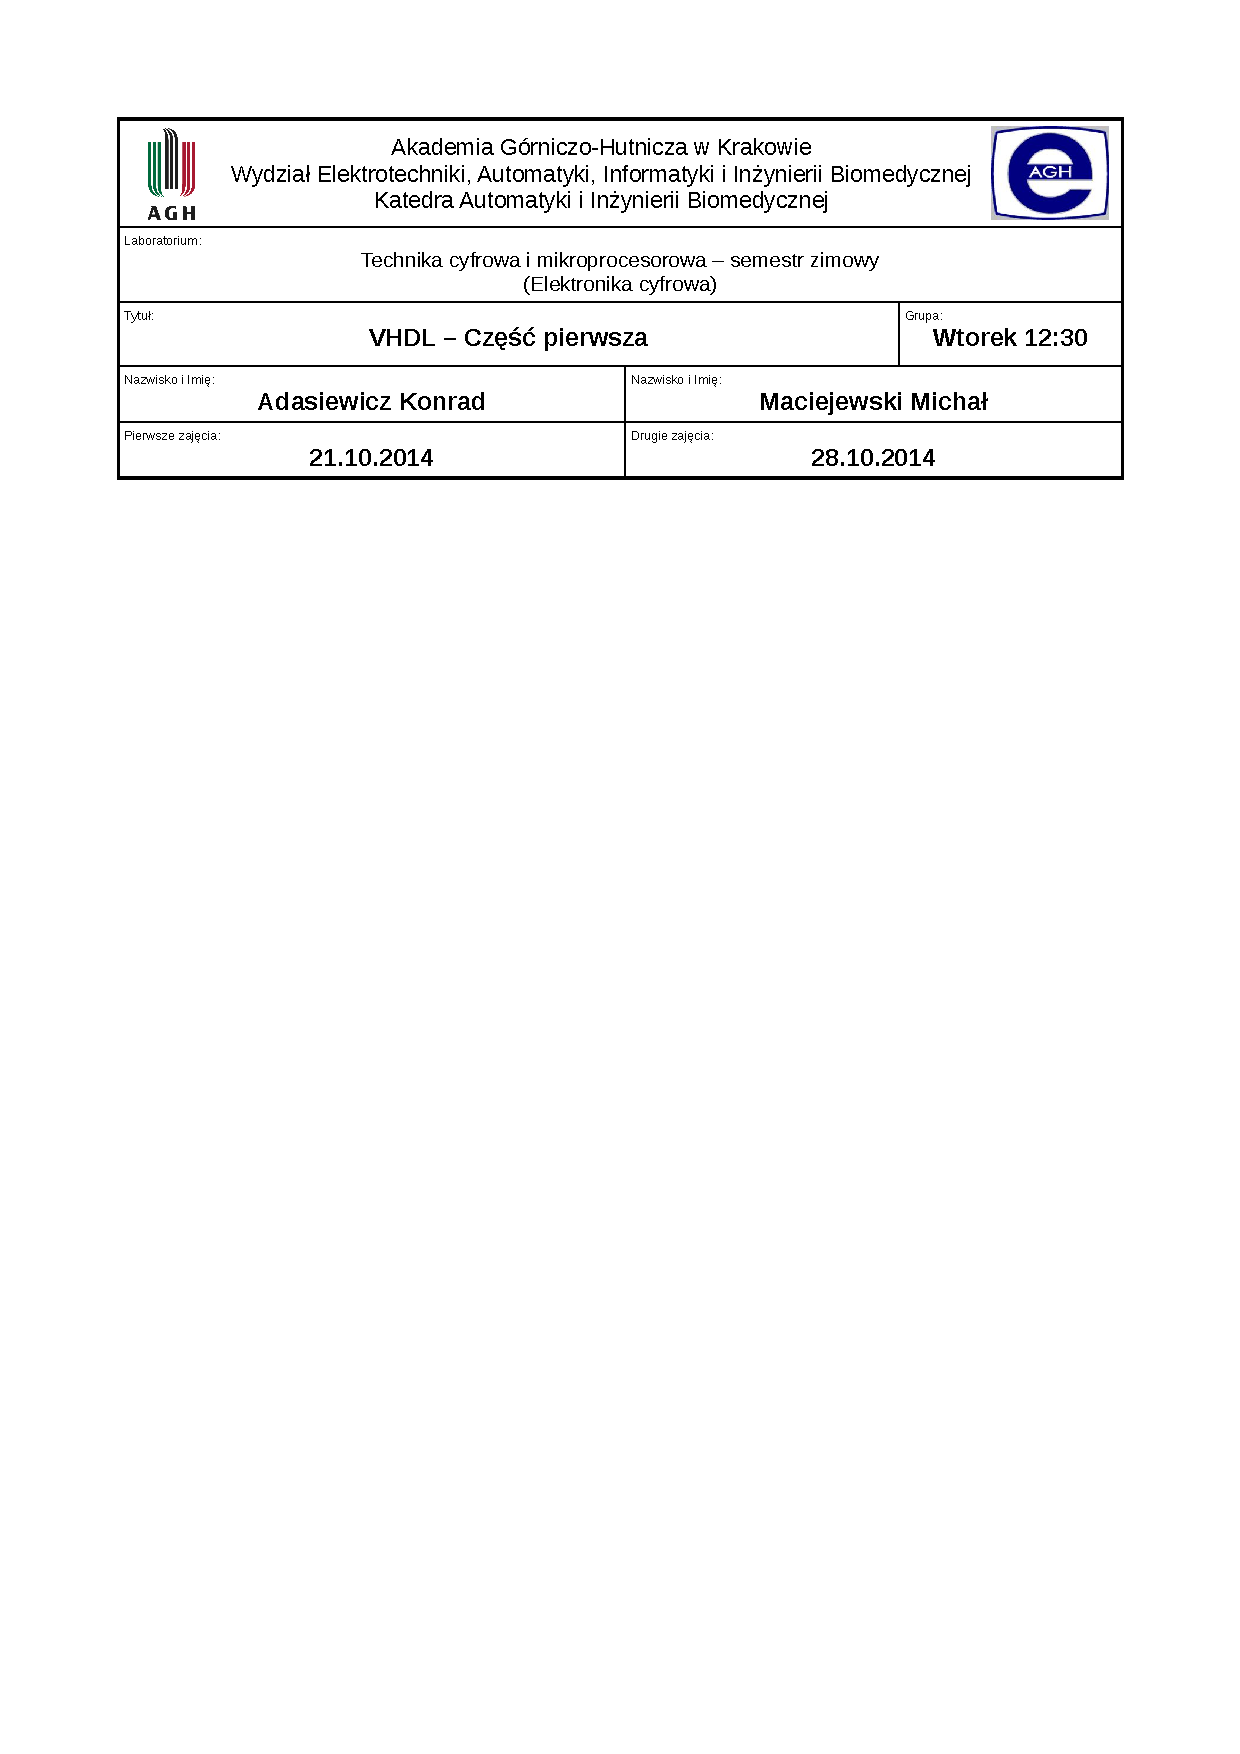
\includegraphics[trim=5cm 21cm 5cm 2cm,width=10cm]{../res/img/table.pdf} 
\end{center}

\begin{lstlisting}[language=VHDL, style=mystyle]
----------------------------------------------------------------------------------
--
--      Kod napisany na potrzeby laboratorium Techniki Mikroprocesorowej
--      Data:       21.10.2014
--      Autorzy:    Konrad Adasiewicz
--                  Michal Maciejewski
-- 
--      Info:       Kod zawiera kilka blokow 'architecture' odnoszacych 
--                  sie do jednego entity, w celu uzycia kodu, niechciane
--                  bloki architecture nalezy wykomentowac
--
----------------------------------------------------------------------------------

-- Used libraries
library IEEE;
use IEEE.STD_LOGIC_1164.ALL;

entity bramki is
    Port (  SWITCH      : in        STD_LOGIC_VECTOR (0 to 3);
            LED         : inout     STD_LOGIC_VECTOR (0 to 5));
end bramki;

-- Implementuje podstawowe dwuwejsciowe funkcje logiczne
-- i wyswietla ich wyniki na diodach LED:
-- (AND, OR, NAND, NOR, XOR, XNOR)
architecture Behavioral of bramki is
begin
    LED(0) <= 	  SWITCH(0) and SWITCH (1);
    LED(1) <= 	  SWITCH(0) or  SWITCH (1);
    LED(2) <= not(SWITCH(0) and SWITCH (1));
    LED(3) <= not(SWITCH(0) or  SWITCH (1));
    LED(4) <= 	  SWITCH(0) xor SWITCH (1);
    LED(5) <= not(SWITCH(0) xor SWITCH (1));
end Behavioral;

-- Implementuje podstawowe trzywejsciowe funkcje logiczne
-- i wyswietla ich wyniki na diodach LED:
-- (AND, OR, NAND, NOR, XOR, XNOR)
architecture Behavioral of bramki is
begin
    LED(0) <= 	  SWITCH(0) and SWITCH (1) and SWITCH (2);
    LED(1) <= 	  SWITCH(0) or  SWITCH (1) or  SWITCH (2);
    LED(2) <= not(SWITCH(0) and SWITCH (1) and SWITCH (2));
    LED(3) <= not(SWITCH(0) or  SWITCH (1) or  SWITCH (2));
    LED(4) <= 	  SWITCH(0) xor SWITCH (1) xor SWITCH (2);
    LED(5) <= not(SWITCH(0) xor SWITCH (1) xor SWITCH (2));
end Behavioral;

-- Jak poprzednio implementuje podstawowe trzywejsciowe
-- funkcje logiczne i wyswietla ich wyniki na diodach LED,
-- dodatkowo ostatni switch blokuje wyjscia LED na stale
-- je gaszac
architecture Behavioral of bramki is
begin
    LED <=  "000000"
        when SWITCH(3) = '0' else
            (   SWITCH(0) and SWITCH (1) and SWITCH (2),
                SWITCH(0) or  SWITCH (1) or  SWITCH (2),
            not(SWITCH(0) and SWITCH (1) and SWITCH (2)),
            not(SWITCH(0) or  SWITCH (1) or  SWITCH (2)),
                SWITCH(0) xor SWITCH (1) xor SWITCH (2),
            not(SWITCH(0) xor SWITCH (1) xor SWITCH (2)));
end Behavioral;

-- Przyklad uzycia operatora konkatenacji:
-- gdy SWITCH(3) = '0' diody led odzwierciedlaja stany 
-- switchy od 0 do 2, w przeciwnym wypadku stany switchy
-- zostaje odzwierciedlony w innej kolejnosci poprzez konkatenacje
-- czesci wektora z jego reszta w innej kolejnosci
architecture Behavioral of bramki is
begin
    LED <=  "000" & SWITCH(0 to 2)
        when SWITCH(3) = '0' else
            "000" & SWITCH(2) & SWITCH(0 to 1);
end Behavioral;
\end{lstlisting}

\newpage

\begin{lstlisting}[language=VHDL, style=mystyle]
----------------------------------------------------------------------------------
--
--      Kod napisany na potrzeby laboratorium Techniki Mikroprocesorowej
--      Data:       28.10.2014
--      Autorzy:    Konrad Adasiewicz
--                  Michal Maciejewski
-- 
--      Info:       Kod zawiera kilka blokow 'architecture' odnoszacych 
--                  sie do jednego entity, w celu uzycia kodu, niechciane
--                  bloki architecture nalezy wykomentowac
--
----------------------------------------------------------------------------------

-- Used libraries
library IEEE;
use IEEE.STD_LOGIC_1164.ALL;
use IEEE.STD_LOGIC_UNSIGNED.ALL;
use IEEE.NUMERIC_STD.ALL;


entity counter is
    Port (      CLK         : in            STD_LOGIC;
                LED         : inout         STD_LOGIC;
                SWITCH      : in            STD_LOGIC_VECTOR (3 downto 0));
end counter;

-- Dioda LED mrugajaca z czestotliwoscia ok
-- 2Hz (z dokladnoscia do mozliwosci osiagniecia
-- rzadanej czestotliwosci z preskalowanego licznika)
architecture arch_counter of counter is
signal DATA : STD_LOGIC_VECTOR (24 downto 0);
begin
   process(CLK)
   begin
       if rising_edge(CLK) then
            -- Inkrementuj licznik przy narastajacym zboczu zegara
            DATA <= DATA + 1;
       end if;
   end process;
   -- Polacz 24 bit licznika z wyjsciem diody
   LED <= DATA(24);
end arch_counter;
 
-- Dioda LED mrugajaca z czestotliwoscia dokladnie
-- 2Hz (2Hz*12500000*2 = 50MHz)
architecture arch_counter of counter is
begin 
   process(CLK)
   variable DATA : integer range 0 to 12500000;
   begin
       if rising_edge(CLK) then
            -- Inkrementuj licznik przy narastajacym zboczu zegara
            DATA := DATA + 1;
            if DATA = 0 then
                -- Przy przepelnieniu licznika zaneguj stan diody
                LED <= not LED;
           end if;
       end if;
   end process;
end arch_counter;

-- Dioda LED modulowana sygnalem PWM o wspolczynniku
-- wypelnienia zadawanym przez switche
architecture arch_counter of counter is
begin
    process(CLK, SWITCH)
    variable DATA : STD_LOGIC_VECTOR (15 downto 0);
    begin
        if rising_edge(CLK) then
            -- Inkrementuj licznik przy narastajacym zboczu zegara
            DATA := DATA + 1;
            if DATA = 0 then
                -- Przy przepelnieniu licznika zaswiec diode
                led <= '1';
            end if;
            if DATA = (SWITCH * X"1000") then
                -- Przy osiagnieciu przez licznik wartosci zaleznej od stanu
                -- switchy zgas diode
                led <= '0';
            end if;
        end if;
    end process;
end arch_counter;
\end{lstlisting}

\end{document}